\documentclass[border = .2cm]{standalone}
\usepackage{tikz}
\usepackage{amsmath}

\begin{document}
  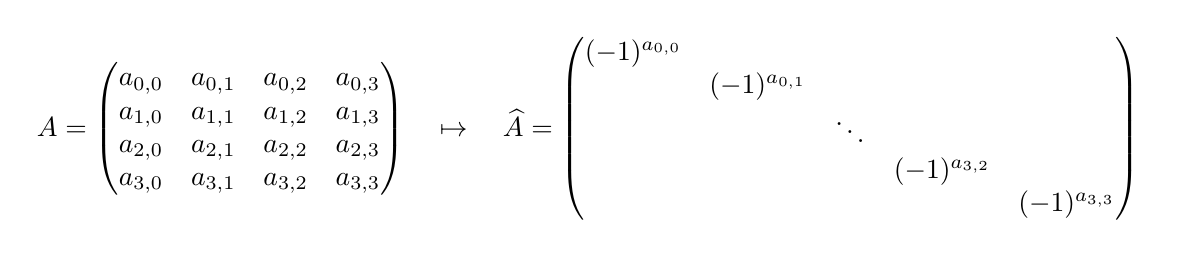
\begin{tikzpicture}
    \node at (0, 0) {$
      A=\begin{pmatrix}
        a_{0, 0} & a_{0, 1} & a_{0, 2} & a_{0, 3}\\
        a_{1, 0} & a_{1, 1} & a_{1, 2} & a_{1, 3}\\
        a_{2, 0} & a_{2, 1} & a_{2, 2} & a_{2, 3}\\
        a_{3, 0} & a_{3, 1} & a_{3, 2} & a_{3, 3}
      \end{pmatrix} \quad\mapsto\quad
      \widehat{A}=\begin{pmatrix}
        (-1)^{a_{0, 0}} \\
        & (-1)^{a_{0, 1}} \\
        & & \ddots \\
        & & & (-1)^{a_{3, 2}} \\
        & & & & (-1)^{a_{3, 3}}
      \end{pmatrix}
    $};
  \end{tikzpicture}
\end{document} 
